\par Realizamos este experimento sobre una red doméstica.

\subsubsection{Fuente $S$}

\par A continuación podemos ver la fuente $S$ propuesta, modelada con los resultados del experimento: \\

\begin{tabular}{ | c | c | c |}
    \hline
    Mensaje & Probabilidad & Información [bits] \\
    \hline
    \textit{Unicast} & 0.848 & 0.237 \\
    \hline
    \textit{Broadcast} & 0.152 & 2.720 \\
    \hline
\end{tabular} \\

\par Entropía de la fuente: 0.614 bits. Entropía máxima: 1 bit.

\par Observamos que la entropía de la fuente es menor que la máxima; las transmisiones \textit{unicast} son significativamente más probables que las \textit{broadcast}.
Esto nos indica que los protocolos de control tienen un bajo impacto en la \textit{performance} de la red.

\subsubsection{Estructura de la red en base a los paquetes ARP}

\par En la figura \ref{ARPcasa} se puede ver el grafo de la red subyacente de mensajes ARP.

\begin{figure*}[ht]
    \centering
    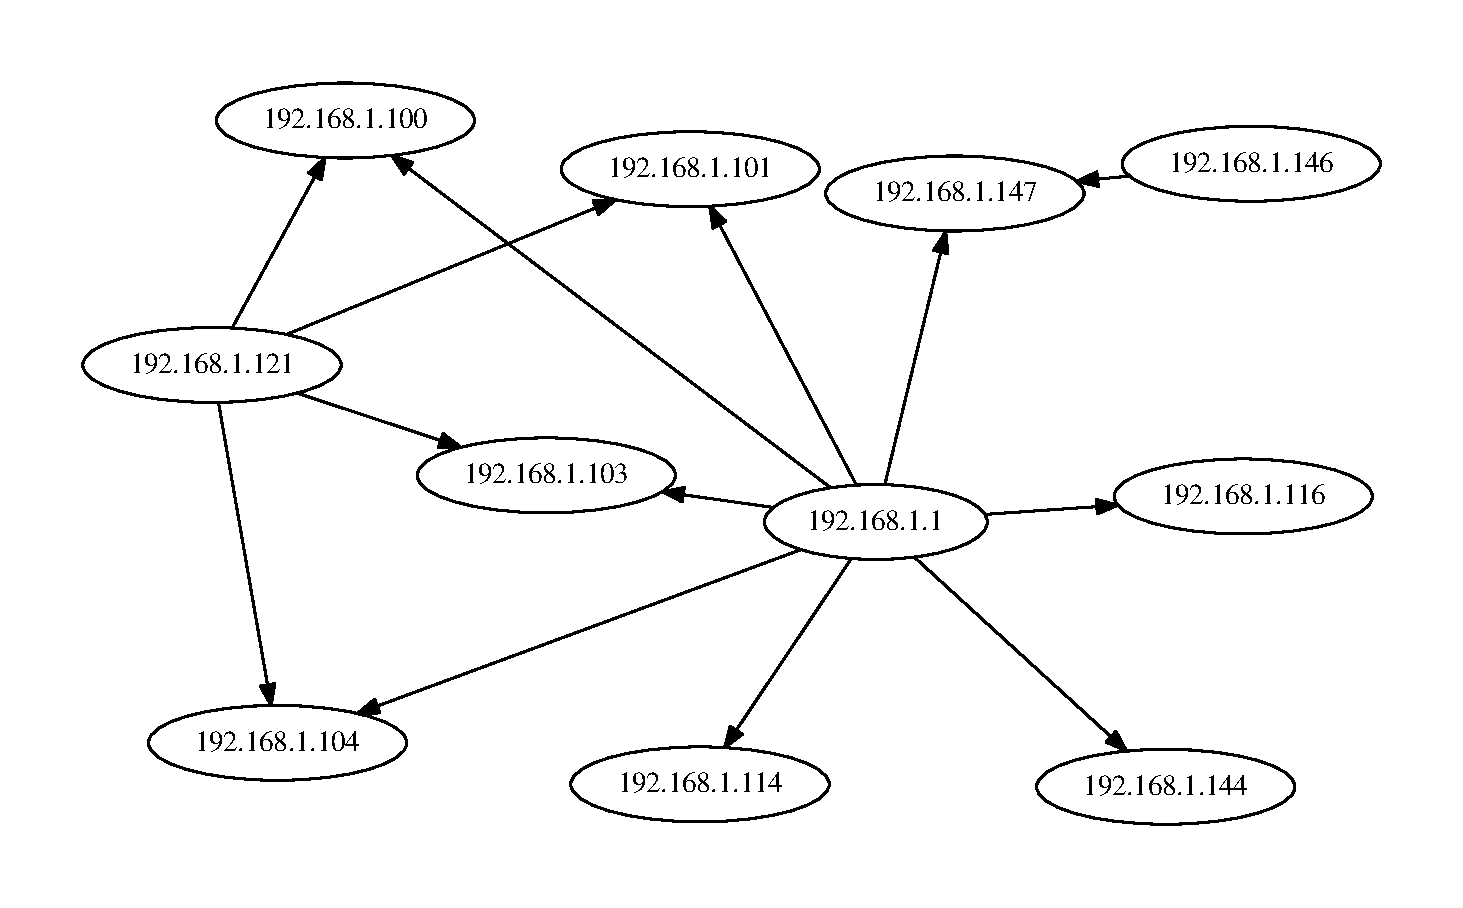
\includegraphics[width=0.9\textwidth]{figuras/casa_grafo.pdf}
    \caption{Grafo de la red subyacente de mensajes ARP en el experimento 3.}\label{ARPcasa}
\end{figure*}

\par Todas las direcciones IP de la red son de la forma 192.168.1.X.
Éstas son direcciones IP privadas\footnote{Todo el rango 192.168.0.0-192.168.255.255 es privado.}.

\par En el grafo se destaca claramente un nodo, el 192.168.1.1.
El vértice 192.169.1.121 también parece destacarse.
Una comparación entre las MAC addresses que acompañan a estas dos direcciones en los paquetes ARP y los diversos dispositivos de la red nos indicó que la 192.168.1.1 corresponde al router de la red, mientras que la 192.168.1.121, a la interfaz de una de las computadoras.

\subsubsection{Fuente $S_1$}

\par En la figura \ref{fig3SinRSinA} podemos ver la información de los mensajes de la fuente $S_1$, sin paquetes repetidos y tomando sólo el \textit{Sender's Protocol Address} de los paquetes.

\par La entropía de la fuente es de 1.24 bits, siendo la máxima 32 bits. 

\begin{figure}
    \centering
    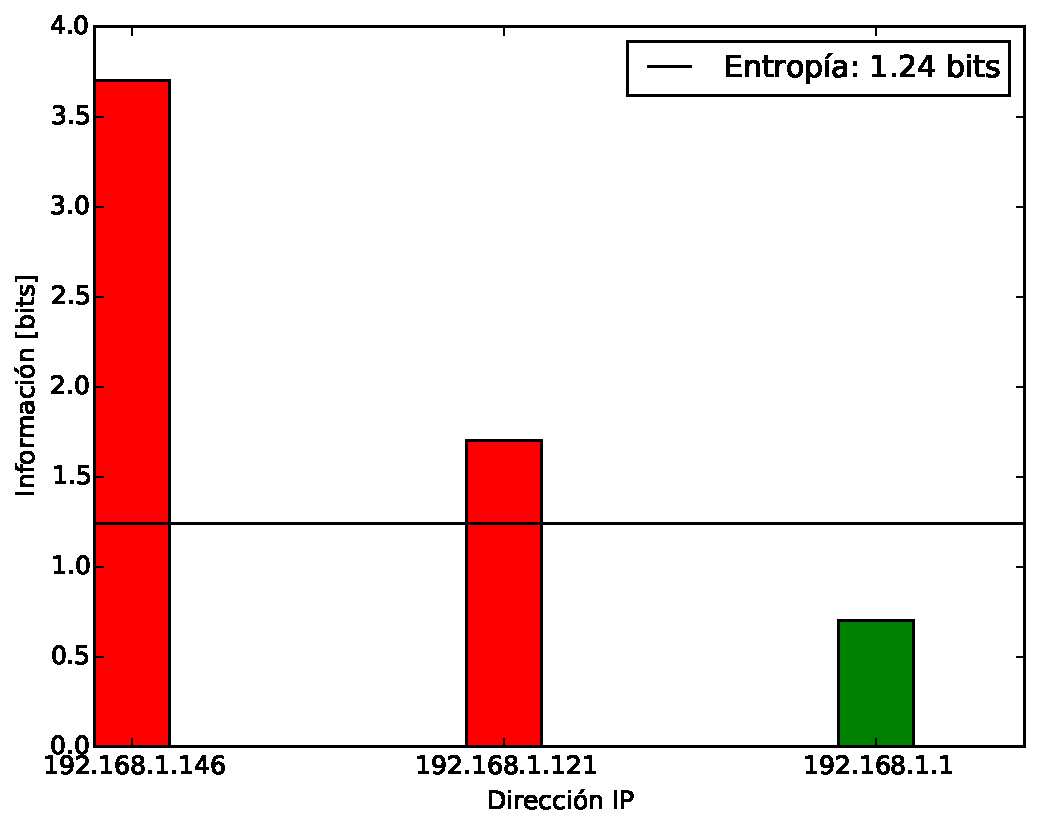
\includegraphics[width=0.45\textwidth]{figuras/casa_figura.pdf}
    \caption{Información de los nodos de la fuente $S_1$ en el experimento 3, sin tomar paquetes repetidos y considerando como mensaje la ocurrencia de una IP en el campo \textit{Sender's Protocol Address} de un paquete ARP \textit{who-has}.}
    \label{fig3SinRSinA}
\end{figure}

\par La fuente clasifica exactamente de la forma deseada: el único nodo distinguido es el correspondiente al router.

\par En la figura \ref{fig3A} podemos ver la información de los mensajes de la fuente $S_1$, sin paquetes repetidos y tomando tanto el campo \textit{Sender's Protocol Address} como el \textit{Target Protocol Address} de los paquetes.

\par La entropía de la fuente es de 3.09 bits, siendo la máxima 32 bits. 

\begin{figure}
    \centering
    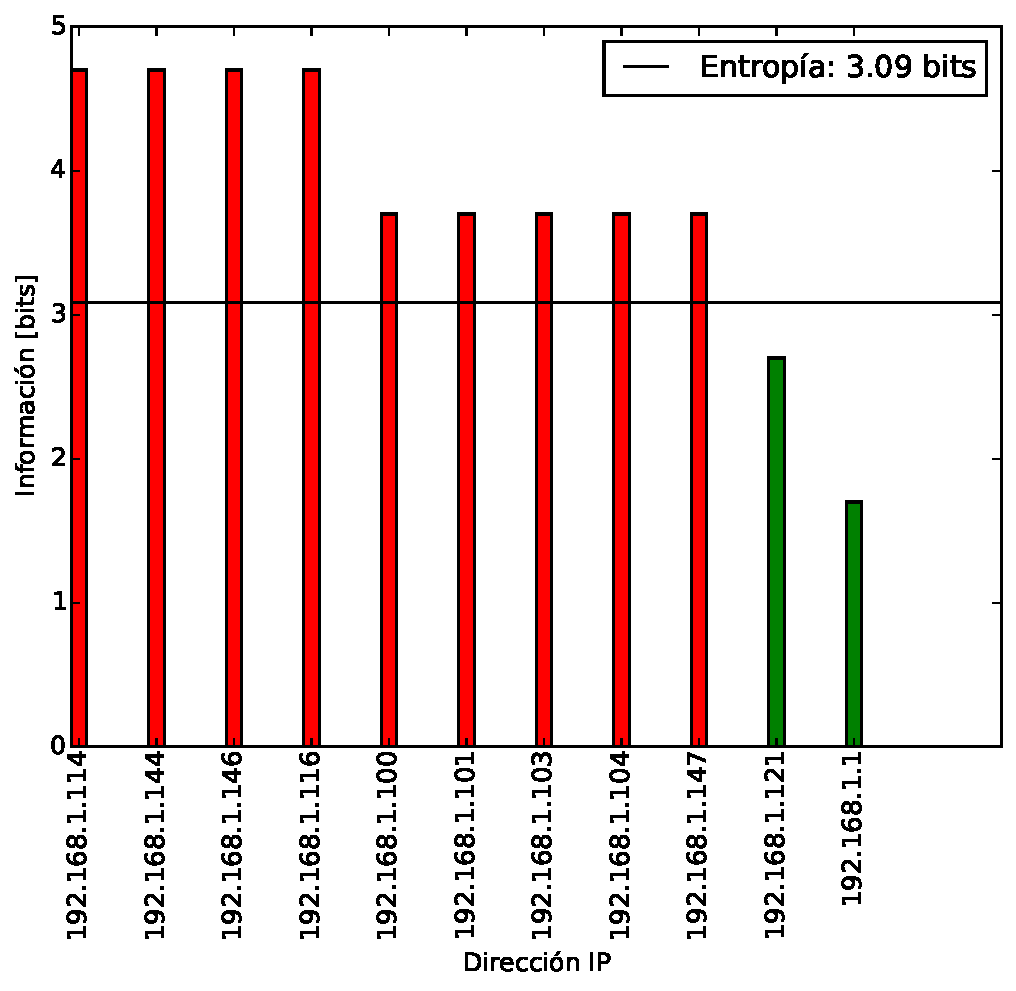
\includegraphics[width=0.45\textwidth]{figuras/casa_figura_ambos.pdf}
    \caption{Información de los nodos de la fuente $S_1$ en el experimento 3, sin tomar paquetes repetidos y considerando como mensaje la ocurrencia de una IP tanto en el campo \textit{Sender's Protocol Address} como en el \textit{Target Protocol Address} de un paquete ARP \textit{who-has}.}
    \label{fig3A}
\end{figure}

\par Al igual que en los otros experimentos, la entropía es mayor al considerar esta fuente.

\par Se presenta un falso negativo, el previamente mencionado nodo 192.168.1.121.
Este resultado es interesante ya que éste actúa exclusivamente como emisor, por lo que la cantidad de veces que aparece en ambas fuentes es igual; la mayor entropía de esta fuente lleva a que sea clasificado como vértice distinguido.
